\documentclass{article}

\usepackage{amsmath}
\usepackage{amsfonts}
\usepackage{amssymb}
\usepackage{graphicx}
\usepackage{float}
\usepackage{geometry}
\usepackage{array}
\usepackage{hyperref}
\renewcommand{\arraystretch}{1.5}

\geometry{
  top=2cm,    % top margin
  bottom=2cm, % bottom margin
  left=2cm, % left margin
  right=2cm % right margin
}

\usepackage[polish]{babel}
\usepackage[utf8]{inputenc}
\usepackage{polski}
\usepackage[T1]{fontenc}

\usepackage{url}

\newenvironment{fact}[1]{%
    \trivlist
    \item[\hskip\labelsep\textbf{Fakt. #1.}]
    \ignorespaces
}{%
    \endtrivlist
}
\newenvironment{theorem}[1]{%
    \trivlist
    \item[\hskip\labelsep\textbf{Theorem. #1.}]
    \ignorespaces
}{%
    \endtrivlist
}

\title{Metody Probabilistyczne i Statystyka}
\author{Zadanie domowe 4}
\date{Rafał Włodarczyk 2025-01-28}

\begin{document}
\maketitle

\tableofcontents

\section{Pomocne twierdzenia}

Przypomnę (sam sobie) pomocne twierdzenia z wykładu.

\subsection{Nierówność Markowa}

\begin{theorem}{Nierówność Markowa} Niech $X: \Omega \rightarrow [0,\infty)$ będzie nieujemną zmienną losową i niech $a\in\mathbb{R}^{+}$. Wówczas:

\[
P(X\geq a) \leq \frac{\mathbf{E}(X)}{a}
\]
\end{theorem}

\subsection{Nierówność Czebyszewa}

\begin{theorem}{Nierówność Czebyszewa} Niech $X: \Omega \rightarrow \mathbb{R}$ będzie zmienną losową, taką, że $\mathbf{E}(X^2) \leq \infty$ i niech $a\in\mathbb{R}^{+}$. Wówczas:
\[
P(|X-\mathbf{E}(X)| \geq a) \leq \frac{\mathbf{var}(X)}{a^2}
\]
\end{theorem}

\section{Zadanie Pierwsze}

\subsection{Obliczenia}

Wiemy, że $X\sim Bin\left(n,p=\frac{1}{2}\right)$, dla rozkładu $Bin\left(n,\frac{1}{2}\right)$ funkcja rozkładu prawdopodobieństwa jest dana wzorem:

\begin{align}
    P(X=k) &= \binom{n}{k}p^k(1-p)^{n-k}, k\in\{0, \dots, n\}\\
\end{align}

\noindent
W celu wyznaczenia aproksymacji dla nierówności Markowa i Czebyszewa
potrzebujemy wyznaczyć $\mathbf{E}(X), \mathbf{var}(X)$:

\begin{align}
    \mathbf{E}(X) &= \sum_{k=0}^{n} k \cdot \binom{n}{k}\cdot \left(\frac{1}{2}\right)^k\cdot \left(\frac{1}{2}\right)^{n-k} =\\
    =\left(\frac{1}{2}\right)^n \sum_{k=0}^{n} \binom{n}{k} k &= \left(\frac{1}{2}\right)^n \cdot n \cdot 2^{n-1} = \frac{n}{2}\\
    \text{oraz } \mathbf{E}(X^2) &= \left(\frac{1}{2}\right)^n \cdot \sum_{k=0}^{n} k^2 \cdot \binom{n}{k} = \left(\frac{1}{2}\right)^n \cdot n(n+1)2^{n-2} = \frac{n(n+1)}{4}\\
    \text{więc } \textbf{var}(X) &= \mathbf{E}(X^2) - (\mathbf{E}(X))^2 = \frac{n}{4}
\end{align}

\noindent

\subsubsection{a) Nierówność Markowa dla $P(X\geq 1 \frac{1}{5} \mathbf{E}(X))$}

\begin{align*}
    P\left(X\geq \frac{6}{5} \mathbf{E}(X)\right) &\leq_{\text{markov}} \frac{\mathbf{E}(X)}{\frac{6}{5}\mathbf{E}(X)} = \frac{5}{6}
\end{align*}

\subsubsection{a) Nierówność Czebyszewa dla $P(X\geq 1 \frac{1}{5} \mathbf{E}(X))$}

\begin{align*}
    P\left(X\geq \frac{6}{5} \mathbf{E}(X)\right) &= P\left(X-\mathbf{E}(X) \geq \frac{1}{5} \mathbf{E}(X)\right)=\\
    =_{\text{sym}} \frac{1}{2}P\left(|X-\mathbf{E}(X)| \geq \frac{1}{5} \mathbf{E}(X) \right) &\leq_{\text{chebyshev}} \frac{1}{2} \frac{\mathbf{var}(X)}{\left[\frac{1}{5}\mathbf{E}(X)\right]^2} = \frac{25\mathbf{var}(X)}{2\mathbf{E}^2(X)} = \frac{25\cdot\frac{n}{4}}{2\cdot \frac{n^2}{4}} = \frac{25}{2n}
\end{align*}

\subsubsection{b) Nierówność Markowa dla $P(|X - \mathbf{E}(X)| \geq \frac{1}{10} \mathbf{E}(X))$}

\begin{align*}
    P\left(|X-\mathbf{E}(X)|\geq \frac{1}{10} \mathbf{E}(X)\right) &= 2 \cdot P\left(X-\mathbf{E}(X)\geq \frac{1}{10} \mathbf{E}(X)\right)=\\
    =_{\text{sym}} 2\cdot P\left(X\geq \frac{11}{10}\mathbf{E}(X)\right) &\leq_{\text{markov}} 2 \cdot \frac{\mathbf{E}(X)}{\frac{11}{10}\mathbf{E}(X)} = \frac{20}{11}
\end{align*}

\subsubsection{b) Nierówność Czebyszewa dla $P(|X - \mathbf{E}(X)| \geq \frac{1}{10} \mathbf{E}(X))$}
\begin{align}
    P\left(|X-\mathbf{E}(X)|\geq \frac{1}{10} \mathbf{E}(X)\right) &\leq_{\text{chebyshev}} \frac{\mathbf{var}(X)}{\left(\frac{1}{10} \mathbf{E}(X)\right)^2} =\\
    = \frac{100\mathbf{var}(X)}{\mathbf{E}^2(X)} &= \frac{100\cdot \frac{n}{4}}{\frac{n^2}{4}} = \frac{100n}{4} \cdot \frac{4}{n^2} = \frac{100}{n}
\end{align}

\subsection{Wyniki}

Dokładne wartości wyliczyłem za pomocą metod numerycznych (program \textit{ex1.py} na końcu dokumentu).

\begin{verbatim}
[~] python ex1.py                                                                                       
Calculations for P(X >= 6/5 E(X))
n = 100, 6/5 * e = 60.00, p = 0.0285830000, markov = 1.20, chebyshev = 0.12
n = 1000, 6/5 * e = 600.00, p = 0.0000000000, markov = 1.20, chebyshev = 0.01
n = 10000, 6/5 * e = 6000.00, p = 0.0000000000, markov = 1.20, chebyshev = 0.00
Calculations for P(|X - E(X)| >= 1/10 E(X))
n = 100, 1/10 * e = 5.00, p = 0.3671530000, markov = 1.82, chebyshev = 1.00
n = 1000, 1/10 * e = 50.00, p = 0.0017020000, markov = 1.82, chebyshev = 0.10
n = 10000, 1/10 * e = 500.00, p = 0.0000000000, markov = 1.82, chebyshev = 0.01
\end{verbatim}

\noindent
Wyniki powyższych obliczeń i symulacji można przedstawić w podanych tabelkach:

\begin{table}[h]
    a)
    \centering
    \begin{tabular}{|l|c|c|c|}
        \hline
        & \textbf{$n = 100$} & \textbf{$n = 1000$} & \textbf{$n = 10000$} \\
        \hline
        \textbf{Markov}   & $\frac{5}{6}$  & $\frac{5}{6}$  & $\frac{5}{6}$  \\
        \hline
        \textbf{Chebyshev} & $\frac{1}{8}$  & $\frac{1}{80}$  & $\frac{1}{800}$  \\
        \hline
        \textbf{Real Value} & $0.028583$ & $small$ & $small$ \\
        \hline
    \end{tabular}
    \caption{Oszacowanie nierówności \textit{a}) dla poszczególnych $n\in\{100,1000,10000\}$}
    \label{tab:markov_chebyshev_a}
\end{table}

\begin{table}[h]
    b)
    \centering
    \begin{tabular}{|l|c|c|c|}
        \hline
        & \textbf{$n = 100$} & \textbf{$n = 1000$} & \textbf{$n = 10000$} \\
        \hline
        \textbf{Markov}   & $\frac{20}{11}$  & $\frac{20}{11}$  & $\frac{20}{11}$  \\
        \hline
        \textbf{Chebyshev} & $1$  & $\frac{1}{10}$  & $\frac{1}{100}$  \\
        \hline
        \textbf{Real Value} & $0.367153$ & $0.001702$ & $small$ \\
        \hline
    \end{tabular}
    \caption{Oszacowanie nierówności \textit{b)} dla poszczególnych $n\in\{100,1000,10000\}$}
    \label{tab:markov_chebyshev_b}
\end{table}

\noindent
Dokładne wartości są trudne do wyznaczenia w języku \textit{python} ze względu na niewielkie ich wartości i niewystarczającą precyzję typu \textit{float}.

\subsection{Wnioski}

Zgodnie z oczekiwaniami dokładniejsze oszacowanie daje nierówność Czebyszewa, jednak w stosunku do rzeczywistej wartości obie wyraźnie prezentują spore niedoszacowanie - rzeczywiście zbadane prawdopodobieństwo jest znacznie mniejsze.


\section{Zadanie Drugie}

\subsection{a) Wyznaczenie numeryczne dystrybuanty empirycznej}

Znamy definicje $S_N = \sum_{n=1}^{N} X_n$, gdzie
$X_n = \begin{cases} 1 & \text{with probability } p = 1/2 \\ -1 & \text{with probability } p = 1/2 \end{cases}$.\\
Oznaczymy liczbę 
\[
l=|\{i\in\{0,1,\dots,N\}: X_i=1\}|
\]
Wtedy widzimy że:

\[
N-l=|\{i\in\{0,1,\dots,N\}: X_i=-1\}|
\]
Wobec tego możemy zapisać:

\[
S_N = 1 \cdot l + (-1) \cdot (N-l) = 2l - N 
\]
Widzimy, że $S_N\in[-n,n]\cap \mathbb{Z_{+}}$. Weźmy $R\sim Bin\left(n,\frac{1}{2}\right)$, zauważmy że
$S_N = 2R-N$ stanowi dobry opis $S_N$. Zgodnie z instrukcją i znanym rozkładem, wykonajmy poniższy program w celu wyznaczenia dystrybuanty empirycznej.

\begin{verbatim}
for n in N:
    values = [k - n for k in 2 * np.random.binomial(n, P, SAMPLES)]

    plt.figure()
    ax = plt.subplot()
    
    res = scipy.stats.ecdf(values)
    res.cdf.plot(ax, label="eCDF", color=ECDF_COLOR)
    
    # get min and max values of the eCDF domain
    min_val = min(values)    
    max_val = max(values)
    ax.plot([-n, min_val], [0, 0], color=ECDF_COLOR) # plot 0 under [-n, min_val]
    ax.plot([max_val, n], [1, 1], color=ECDF_COLOR) # plot 1 over [max_val, n]

    ax.set_title(f"Empirical CDF of $S_{{{n}}}$")
    ax.set_xlabel(f"X")
    ax.set_ylabel(f"$S_{{{n}}}$")

    # b) Plot equivalent normal distribution (mu = 0, sigma = sqrt(n))
    mu = 0
    sigma = np.sqrt(n)
    x = np.linspace(-n, n, SAMPLES)
    ax.plot(x, scipy.stats.norm.cdf(x, mu, sigma), label="Normal CDF", color=NORM_COLOR)
    ax.legend()
\end{verbatim}

\subsection{b) Aproksymacja rozkładem normalnym}

Rozkład prawdopodobieństwa jest wyznaczony przez funkcję masy:
\[
P(S_N = 2l - N) = \binom{N}{l}p^l(1-p)^{N-l}
\]
Jest to funkcja masy prawdopodobieństwa, która reprezentuje rozkład dwumianowy, dla którego znane są wartości $\mathbf{E}(X)$ oraz $\mathbf{var}(X)$:
\begin{enumerate}
    \item $\mathbf{E}(S_N) = \sum_i\mathbf{E}(X_i) = 0$
    \item $\mathbf{var}(S_N) = \sum_i\mathbf{var}(X_i) = N \cdot 1 = N$
\end{enumerate}
Wobec tego możemy aproksymować $S_N$ rozkładem normalnym o parametrach $\mathcal{N}\left(0,\sqrt{N}\right)$

\subsection{a,b) Wygenerowane wykresy $N\in\{5,15,15,20,25,30\}$}

\begin{figure}[H]
    \centering
        \begin{minipage}{0.24\textwidth}
        \centering
        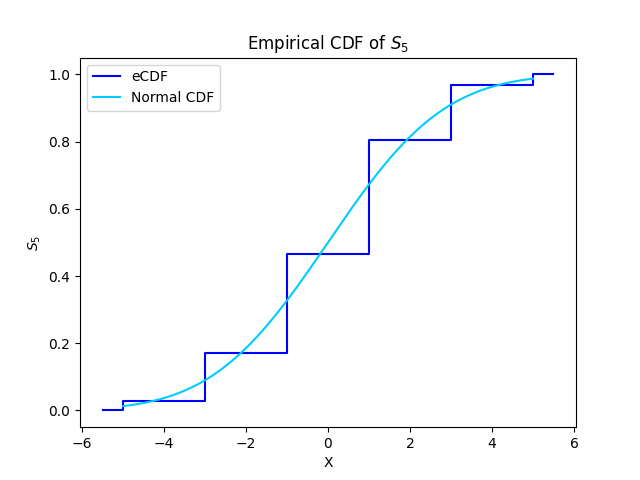
\includegraphics[width=\linewidth]{ex2/ex2_5.png}
        \caption{$N=5$}
    \end{minipage}
        \begin{minipage}{0.24\textwidth}
        \centering
        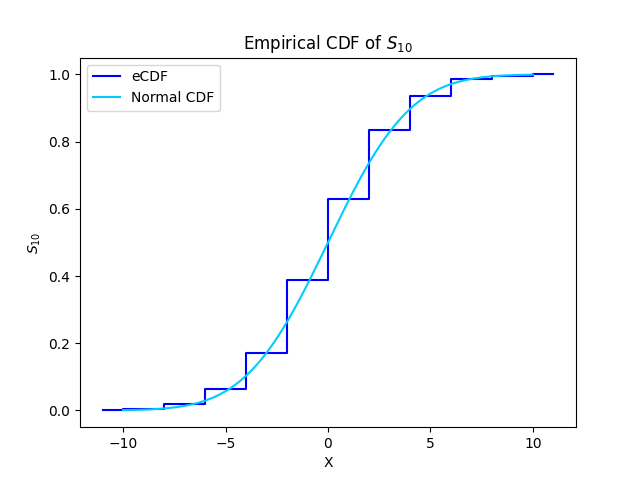
\includegraphics[width=\linewidth]{ex2/ex2_10.png}
        \caption{$N=10$}
    \end{minipage}
        \begin{minipage}{0.24\textwidth}
        \centering
        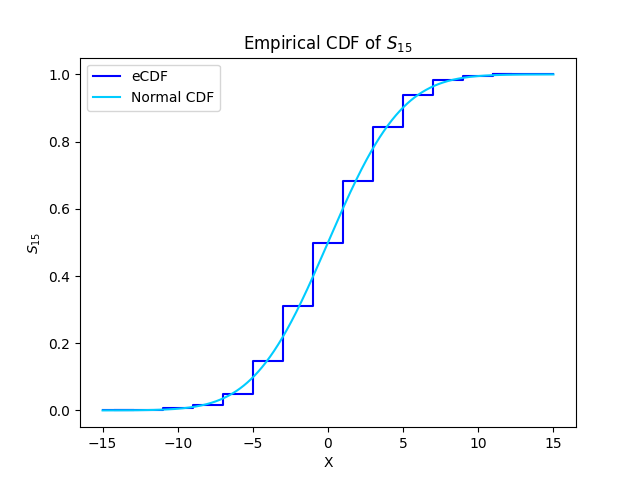
\includegraphics[width=\linewidth]{ex2/ex2_15.png}
        \caption{$N=15$}
    \end{minipage}
\end{figure}

\begin{figure}[H]
    \centering
        \begin{minipage}{0.24\textwidth}
        \centering
        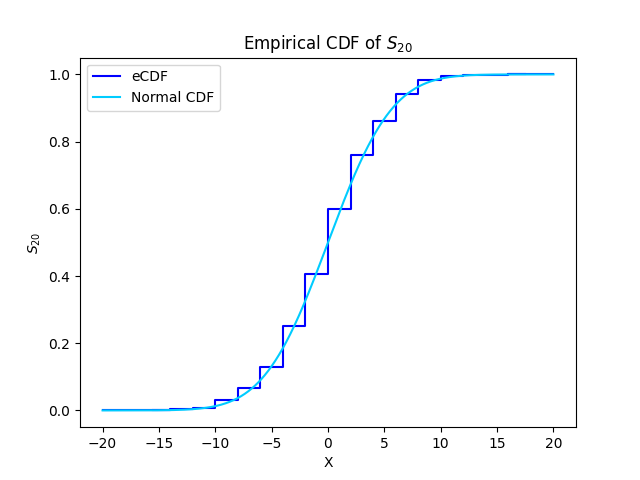
\includegraphics[width=\linewidth]{ex2/ex2_20.png}
        \caption{$N=20$}
    \end{minipage}
        \begin{minipage}{0.24\textwidth}
        \centering
        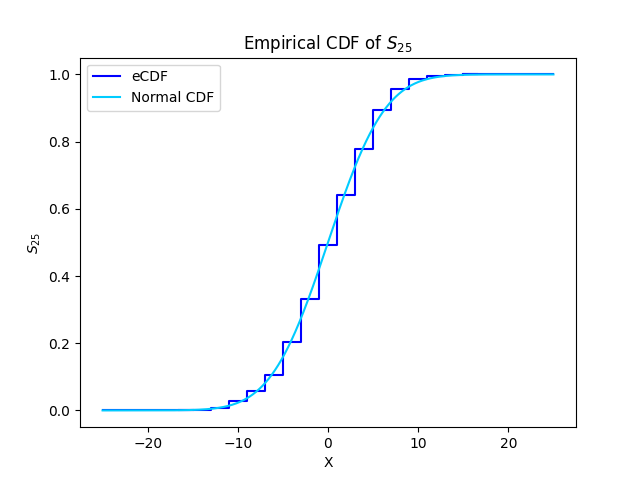
\includegraphics[width=\linewidth]{ex2/ex2_25.png}
        \caption{$N=25$}
    \end{minipage}
        \begin{minipage}{0.24\textwidth}
        \centering
        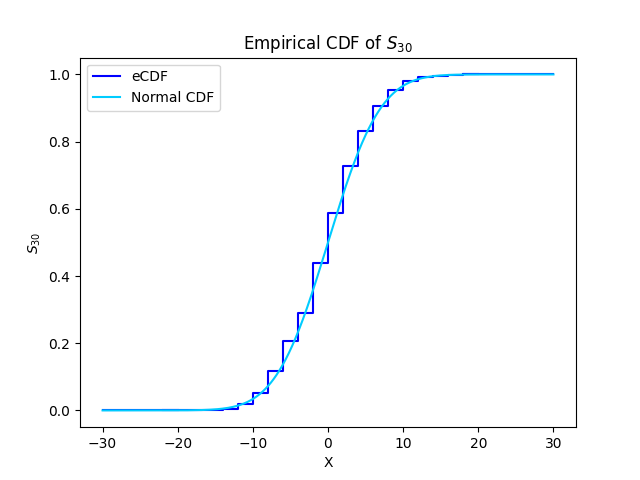
\includegraphics[width=\linewidth]{ex2/ex2_30.png}
        \caption{$N=30$}
    \end{minipage}
\end{figure}

\subsection{c) Wykres dla $N=100$}

\begin{figure}[H]
  \centering
        \begin{minipage}{0.49\textwidth}
        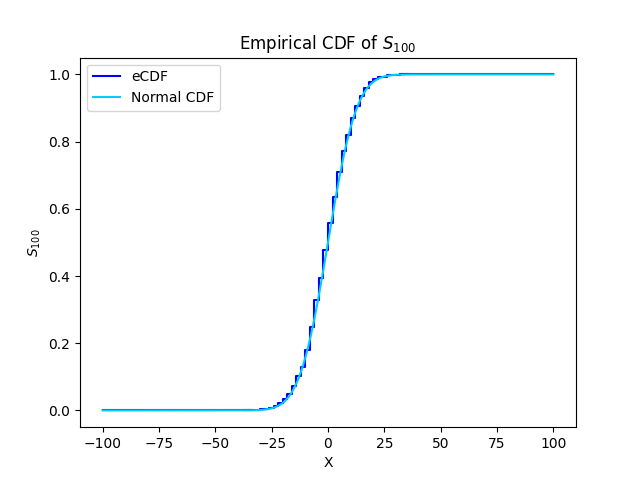
\includegraphics[width=\linewidth]{ex2/ex2_100.png}
        \caption{$N=100$}
    \end{minipage}
\end{figure}

\subsection{Wyniki}

Wykresy dystrybuant empirycznych i dystrybuanty dopasowanego do nich rozkładów normalnych cechują się wysokim podobieństwem. Dodatkowo wraz ze wzrostem $N$ obserwujemy znaczące zbliżanie się wykresu dystrybuanty empirycznej do wykresu odpowiadającego rozkładu normalnego.

\subsection{Wnioski}

Zadany rozkład $S_N$ (liniowo przekształcony rozkład dwumianowy) możemy sukcesywnie aproksymować za pomocą rozkładu normalnego o odpowiednich parametrach.

\section{Zadanie Trzecie}

Weźmy $S_N = \sum_{n=1}^{N} X_n$ jak wyżej oraz $X_n = \begin{cases} 1 & \text{with probability } 1/2 \\ -1 & \text{with probability } 1/2 \end{cases}$ jak wyżej. Wprowadźmy następujące parametry
\begin{enumerate}
    \item $D_{n} = 1 (S_n > 0 \lor S_{n-1} > 0), n = 1, 2, ...$
    \item $L_{N} = \sum_{n=1}^{N} D_{n}, N \in \mathbb{N}$ - a sequence to be analyzed
    \item $P_{N} = \frac{L_{N}}{N}$ - the fraction of positive terms in the sequence $L_{N}$
\end{enumerate}

\subsection{a,b) Realizacja symulacji}

Symulacja została zrealizowana za pomocą następującego kodu.

\begin{verbatim}
# k individual simulations for each n
for i in range(k):
    values = R * np.random.binomial(1, P, n)

    l = 0
    state = 0
    prev_state = 0
    for j in range(n):
        prev_state = state
        if values[j] > 0:
            state += 1
        else:
            state -= 1

        if state > 0 or prev_state > 0:
            l += 1
        
    p = l / n
    print(f"n = {n}, l = {l}, p = {p}")
\end{verbatim}

\noindent
Widzimy, że dla ułatwienia posłużyłem się rozkładem $Bin\left(1,\frac{1}{2}\right)$ i zmapowałem wartość zmiennej losowej jako $(0 \rightarrow -1), (1\rightarrow 1)$.
\subsection{c) Normalizacja i histogram}

\textit{matplotlib} pozwala na uwzględnienie parametrów \textbf{bins=20} oraz \textbf{density=True} (normalizacja).

\begin{verbatim}
plt.hist(probs, bins=20, edgecolor='black', alpha=0.7, density=True, label="P Density")
plt.title(f'Histogram of $P_{{{n}}}$')
plt.xlabel(f'$P_{{{n}}}$')
plt.ylabel('Density')
\end{verbatim}

\subsection{d) Wykresem gęstości rozkładu arcsin}

Wyznaczona gęstość rozkładu dla arcsin w zadaniu 5L8 wyniosła:

\[
p_x = \frac{1}{\pi \cdot \sqrt{x\cdot (1-x)}}
\]

\subsection{Wykresy}

\begin{figure}[H]
    \centering
        \begin{minipage}{0.24\textwidth}
        \centering
        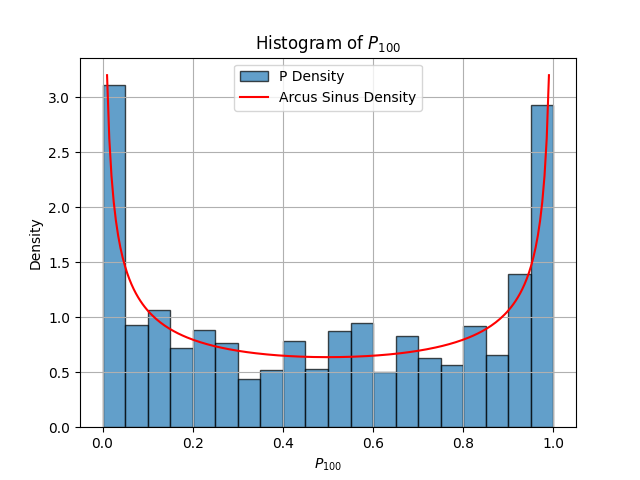
\includegraphics[width=\linewidth]{ex3/ex3_100.png}
        \caption{$N=100$}
    \end{minipage}
        \begin{minipage}{0.24\textwidth}
        \centering
        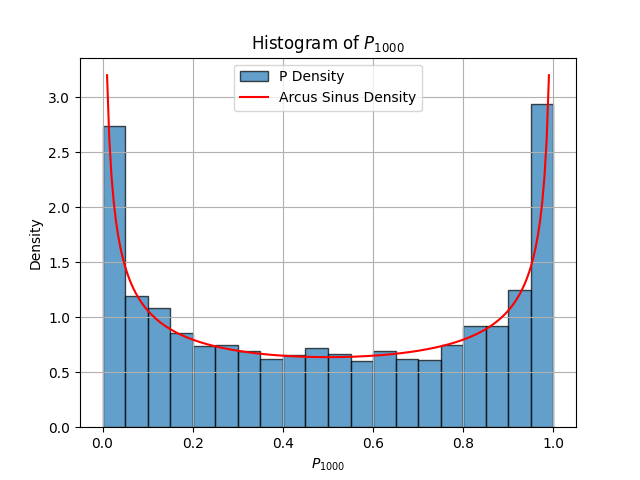
\includegraphics[width=\linewidth]{ex3/ex3_1000.png}
        \caption{$N=1000$}
    \end{minipage}
        \begin{minipage}{0.24\textwidth}
        \centering
        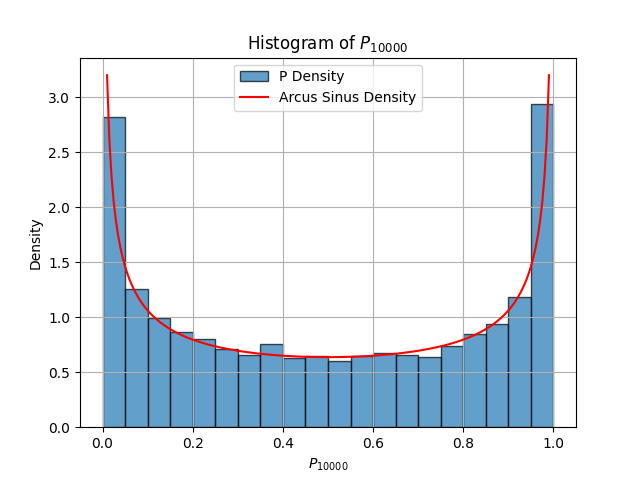
\includegraphics[width=\linewidth]{ex3/ex3_10000.png}
        \caption{$N=10000$}
    \end{minipage}
\end{figure}


\subsection{Wyniki}

Widzimy, że wraz ze wzrostem $N$ wartości poszczególnych kolumn histogramu zbliżają się do wykresu gęstości rozkładu arcsin.

\subsection{Wnioski}

Gęstość rozkładu arcsin w dobry sposób przybliża histogram rozkładu $(P_N^{(1)},\dots,P_N^{(k)})$. 

\section{Zadanie Czwarte}

\subsection{a,b) Idea testów statystycznych}

Zapoznałem się z opisaną ideą, oraz pobieżnie ze specyfikacją testów NIST. Ponadto znalazłem 
\href{https://csrc.nist.gov/projects/random-bit-generation/documentation-and-software/guide-to-the-statistical-tests}{dobry artykuł NIST opisujący każdy z testów}.

\subsection{c) Wykonanie testów}

Wyniki testów wskazują na wysoką zdolność przyzwoitych generatorów PRNG - Mersenne Twister or podanych na stronie przez Zsolta Molnara do sukcesywnego przechodzenia testów podobnych do testów NIST. Część testów, szczególnie te ostatnie zwracały sporo błędów. Zaobserwowałem, że większe ciągi bitów generują mniej błędów w kilku pierwszych testach, stąd decyzja o wyborze pierwszych $1000000$ bitów z każdego generatora wykorzystanego przeze mnie w pythonie.

\newpage

\begin{enumerate}
    \item "Słaby" generator liczb losowych. Napisałem prosty generator $LCM$ w języku \textit{python}, którego wynik pierwszych $1000000$ bitów następnie skopiowałem do schowka i wkleiłem do strony Zsolta Molnara. 
    \begin{figure}[H]
    \centering
    \begin{minipage}{0.6\textwidth}
        \begin{verbatim}
import random
import pyperclip

n = 1_000_000

rand = ''.join([bin(b)[2:] for b in random.randbytes(n)])
print(rand[0:n])

pyperclip.copy(rand)
print("copied to clipboard.")
        \end{verbatim}
    \end{minipage}
    \hfill
    \begin{minipage}{0.35\textwidth}
        \centering
        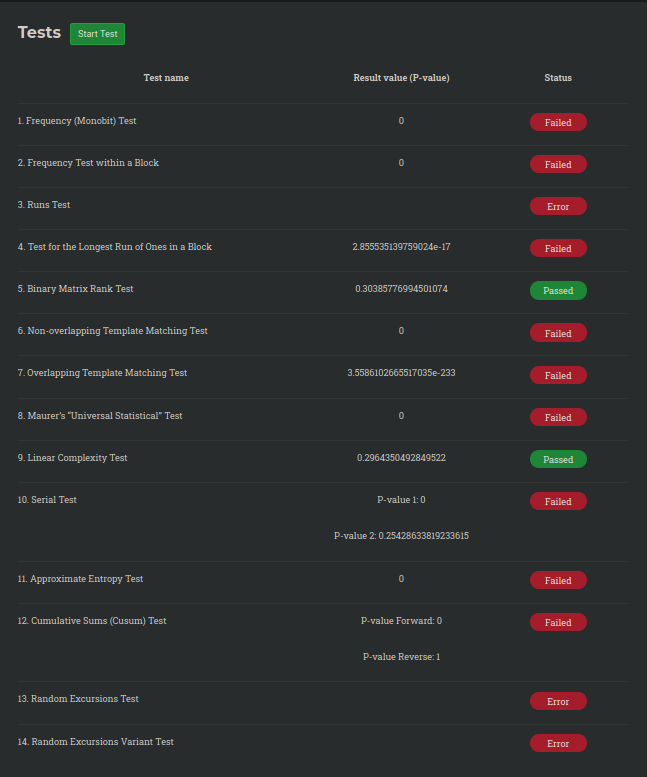
\includegraphics[width=\linewidth]{test4-1.png}
        \caption{Test "Słabego" generatora}
    \end{minipage}
    \end{figure}
    \item "Przyzwoity" generator liczb losowych. Wykorzystałem generator Mersenne Twister, z którego ponownie stworzyłem ciąg pierwszych $1000000$ bitów i wkleiłem do strony Zsolta Molnara.
    \begin{figure}[H]
    \centering
    \begin{minipage}{0.6\textwidth}
        \begin{verbatim}
    from numpy.random import Generator, MT19937, SeedSequence
    import pyperclip
    
    n = 1_000_000
    
    seed = SeedSequence(96243756298)
    rg = Generator(MT19937(seed))
    rand = rg.integers(2, size=n)
    rand = ''.join([str(i) for i in rand])
    print(rand)
    
    pyperclip.copy(rand)
    print("copied to clipboard.")
            \end{verbatim}
        \end{minipage}
        \hfill
        \begin{minipage}{0.35\textwidth}
            \centering
            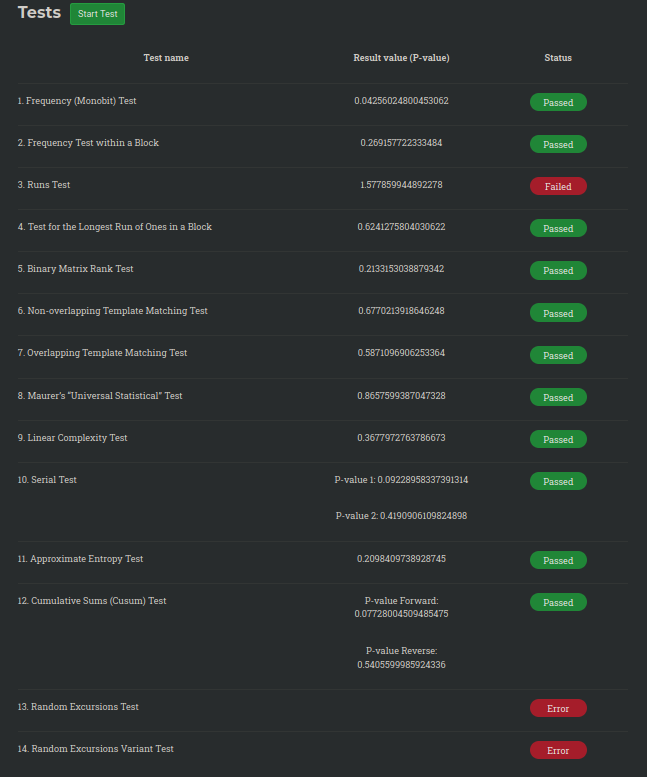
\includegraphics[width=\linewidth]{test4-2.png}
            \caption{Test "Przyzwoitego" Generatora}
        \end{minipage}
    \end{figure}
    \item JavaScript pseudo RNG - Wyklikałem w GUI strony Zsolta Molnara, generując ciąg bitów.
    \begin{figure}[H]
        \centering
        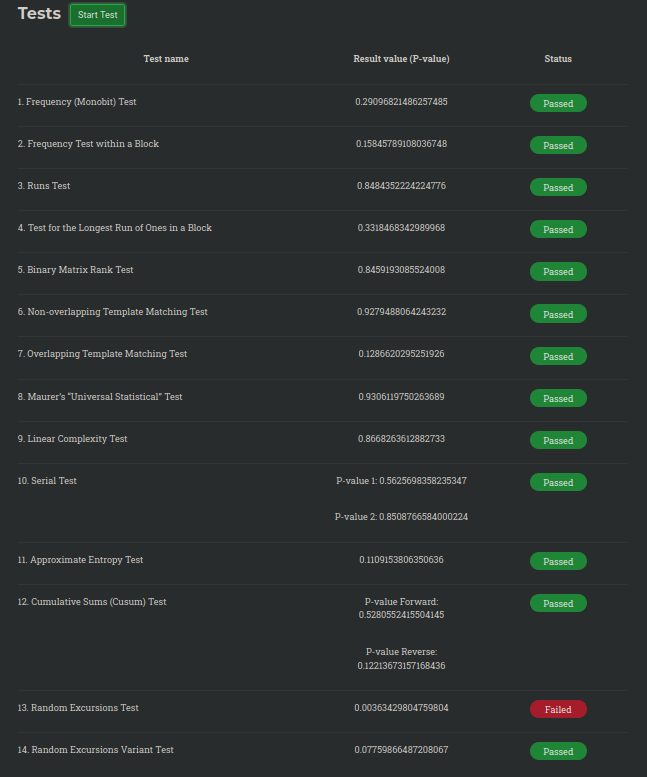
\includegraphics[width=0.4\linewidth]{test4-3.png}
        \caption{Test JavaScript pseudo RNG}
    \end{figure}
\end{enumerate}


\subsection{d) Źródło doskonałej losowości}

Kubuś Puchatek nie może mieć gwarancji na każdowe uzyskanie pozytywnych wyników z każdego testu. Możemy tu powołać się na artykuł:

\begin{itemize}
    \item \href{http://romjist.ro/content/pdf/02-msys.pdf}{Marton, Kinga, and Alin Suciu. "On the interpretation of results from the NIST statistical test suite." Science and Technology 18.1 (2015): 18-32.}
\end{itemize}

W którym opisano proces interpretacji wyników przeprowadzanych testów NIST. Przechodząc do konkluzji podanego artykułu możemy wyczytać, że:

\begin{itemize}
    \item \textit{The NIST STS suggests to consider data to be random if all tests are
passed – yet even truly random data shows a high probability (80\%) of failing at least
one NIST STS test.}
\end{itemize}

\noindent
Zobaczmy, że jeśli istotnie szansa na niezaliczenie testu, w wyniku błędu, którym te testy są obarczone (np $u=1\%$), to istotnie wykonanie pełnego zestawu testów w liczbie $15$ sprawia iż całościowe prawdopodobieństwo niezaliczenia wszystkich testów sprowadza się do zauważalnej wartości na przedziale $[0,1]$ (dla mojego założonego $u$, $(1-u)^{15}\approx 14\%$). Istnieje zatem szereg szczególnych przypadków (kombinacji zaliczeń testów) dla których owe testy, sprawdzające struktury bitowe mogą wywołać tzw \textit{false postive}, czyli określić idealny ciąg Kubusia Puchatka jako wygenerowany za pomocą nieidealnie losowego źródła bitów.


\end{document}